\PassOptionsToPackage{unicode=true}{hyperref} % options for packages loaded elsewhere
\PassOptionsToPackage{hyphens}{url}
%
\documentclass[ignorenonframetext,]{beamer}
\usepackage{pgfpages}
\setbeamertemplate{caption}[numbered]
\setbeamertemplate{caption label separator}{: }
\setbeamercolor{caption name}{fg=normal text.fg}
\beamertemplatenavigationsymbolsempty
% Prevent slide breaks in the middle of a paragraph:
\widowpenalties 1 10000
\raggedbottom
\setbeamertemplate{part page}{
\centering
\begin{beamercolorbox}[sep=16pt,center]{part title}
  \usebeamerfont{part title}\insertpart\par
\end{beamercolorbox}
}
\setbeamertemplate{section page}{
\centering
\begin{beamercolorbox}[sep=12pt,center]{part title}
  \usebeamerfont{section title}\insertsection\par
\end{beamercolorbox}
}
\setbeamertemplate{subsection page}{
\centering
\begin{beamercolorbox}[sep=8pt,center]{part title}
  \usebeamerfont{subsection title}\insertsubsection\par
\end{beamercolorbox}
}
\AtBeginPart{
  \frame{\partpage}
}
\AtBeginSection{
  \ifbibliography
  \else
    \frame{\sectionpage}
  \fi
}
\AtBeginSubsection{
  \frame{\subsectionpage}
}
\usepackage{lmodern}
\usepackage{amssymb,amsmath}
\usepackage{ifxetex,ifluatex}
\usepackage{fixltx2e} % provides \textsubscript
\ifnum 0\ifxetex 1\fi\ifluatex 1\fi=0 % if pdftex
  \usepackage[T1]{fontenc}
  \usepackage[utf8]{inputenc}
  \usepackage{textcomp} % provides euro and other symbols
\else % if luatex or xelatex
  \usepackage{unicode-math}
  \defaultfontfeatures{Ligatures=TeX,Scale=MatchLowercase}
\fi
% use upquote if available, for straight quotes in verbatim environments
\IfFileExists{upquote.sty}{\usepackage{upquote}}{}
% use microtype if available
\IfFileExists{microtype.sty}{%
\usepackage[]{microtype}
\UseMicrotypeSet[protrusion]{basicmath} % disable protrusion for tt fonts
}{}
\IfFileExists{parskip.sty}{%
\usepackage{parskip}
}{% else
\setlength{\parindent}{0pt}
\setlength{\parskip}{6pt plus 2pt minus 1pt}
}
\usepackage{hyperref}
\hypersetup{
            pdftitle={Graph traversal and Path-finding Algorithms used in Video Games},
            pdfauthor={Marius Rabenarivo},
            pdfborder={0 0 0},
            breaklinks=true}
\urlstyle{same}  % don't use monospace font for urls
\newif\ifbibliography
\usepackage{graphicx,grffile}
\makeatletter
\def\maxwidth{\ifdim\Gin@nat@width>\linewidth\linewidth\else\Gin@nat@width\fi}
\def\maxheight{\ifdim\Gin@nat@height>\textheight\textheight\else\Gin@nat@height\fi}
\makeatother
% Scale images if necessary, so that they will not overflow the page
% margins by default, and it is still possible to overwrite the defaults
% using explicit options in \includegraphics[width, height, ...]{}
\setkeys{Gin}{width=\maxwidth,height=\maxheight,keepaspectratio}
\setlength{\emergencystretch}{3em}  % prevent overfull lines
\providecommand{\tightlist}{%
  \setlength{\itemsep}{0pt}\setlength{\parskip}{0pt}}
\setcounter{secnumdepth}{0}

% set default figure placement to htbp
\makeatletter
\def\fps@figure{htbp}
\makeatother


\title{Graph traversal and Path-finding Algorithms used in Video Games}
\author{Marius Rabenarivo}
\date{}

\begin{document}
\frame{\titlepage}

\begin{frame}

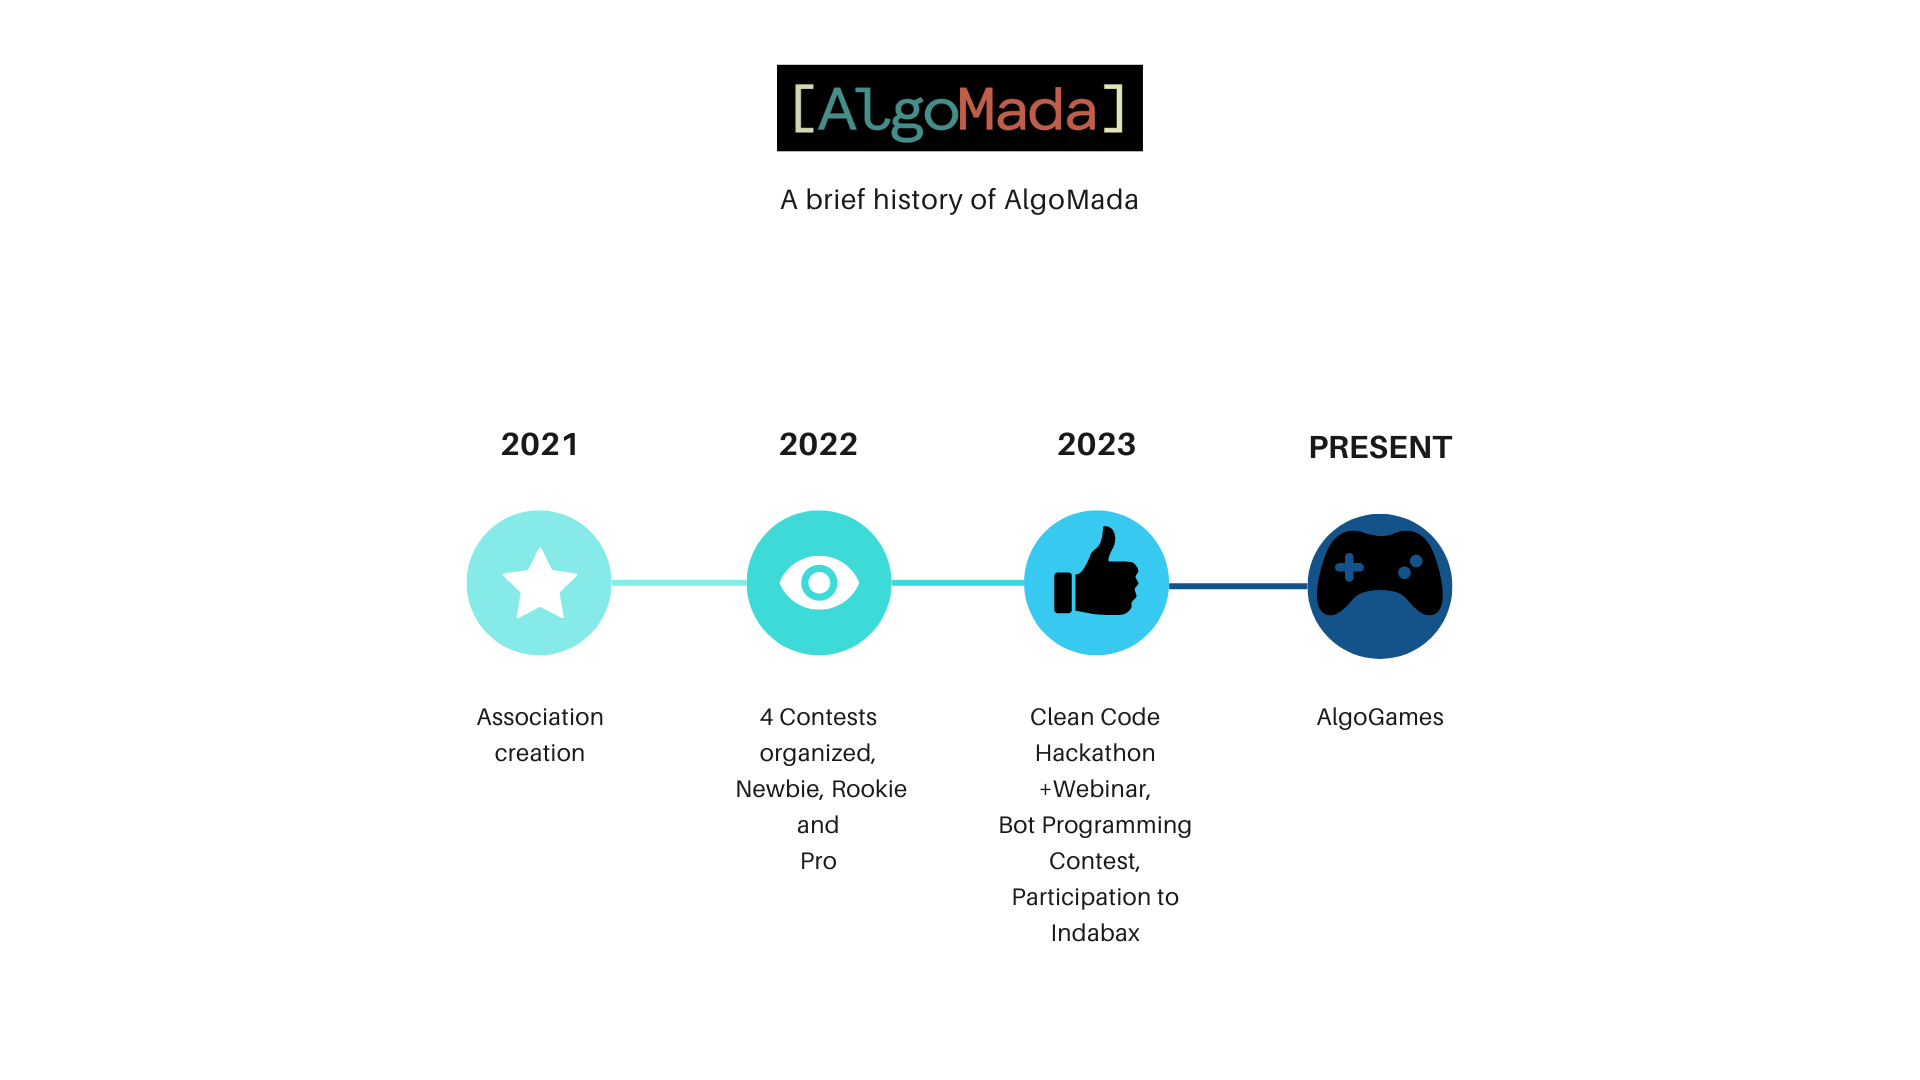
\includegraphics{AlgoMada.png}

\end{frame}

\begin{frame}{About me}
\protect\hypertarget{about-me}{}

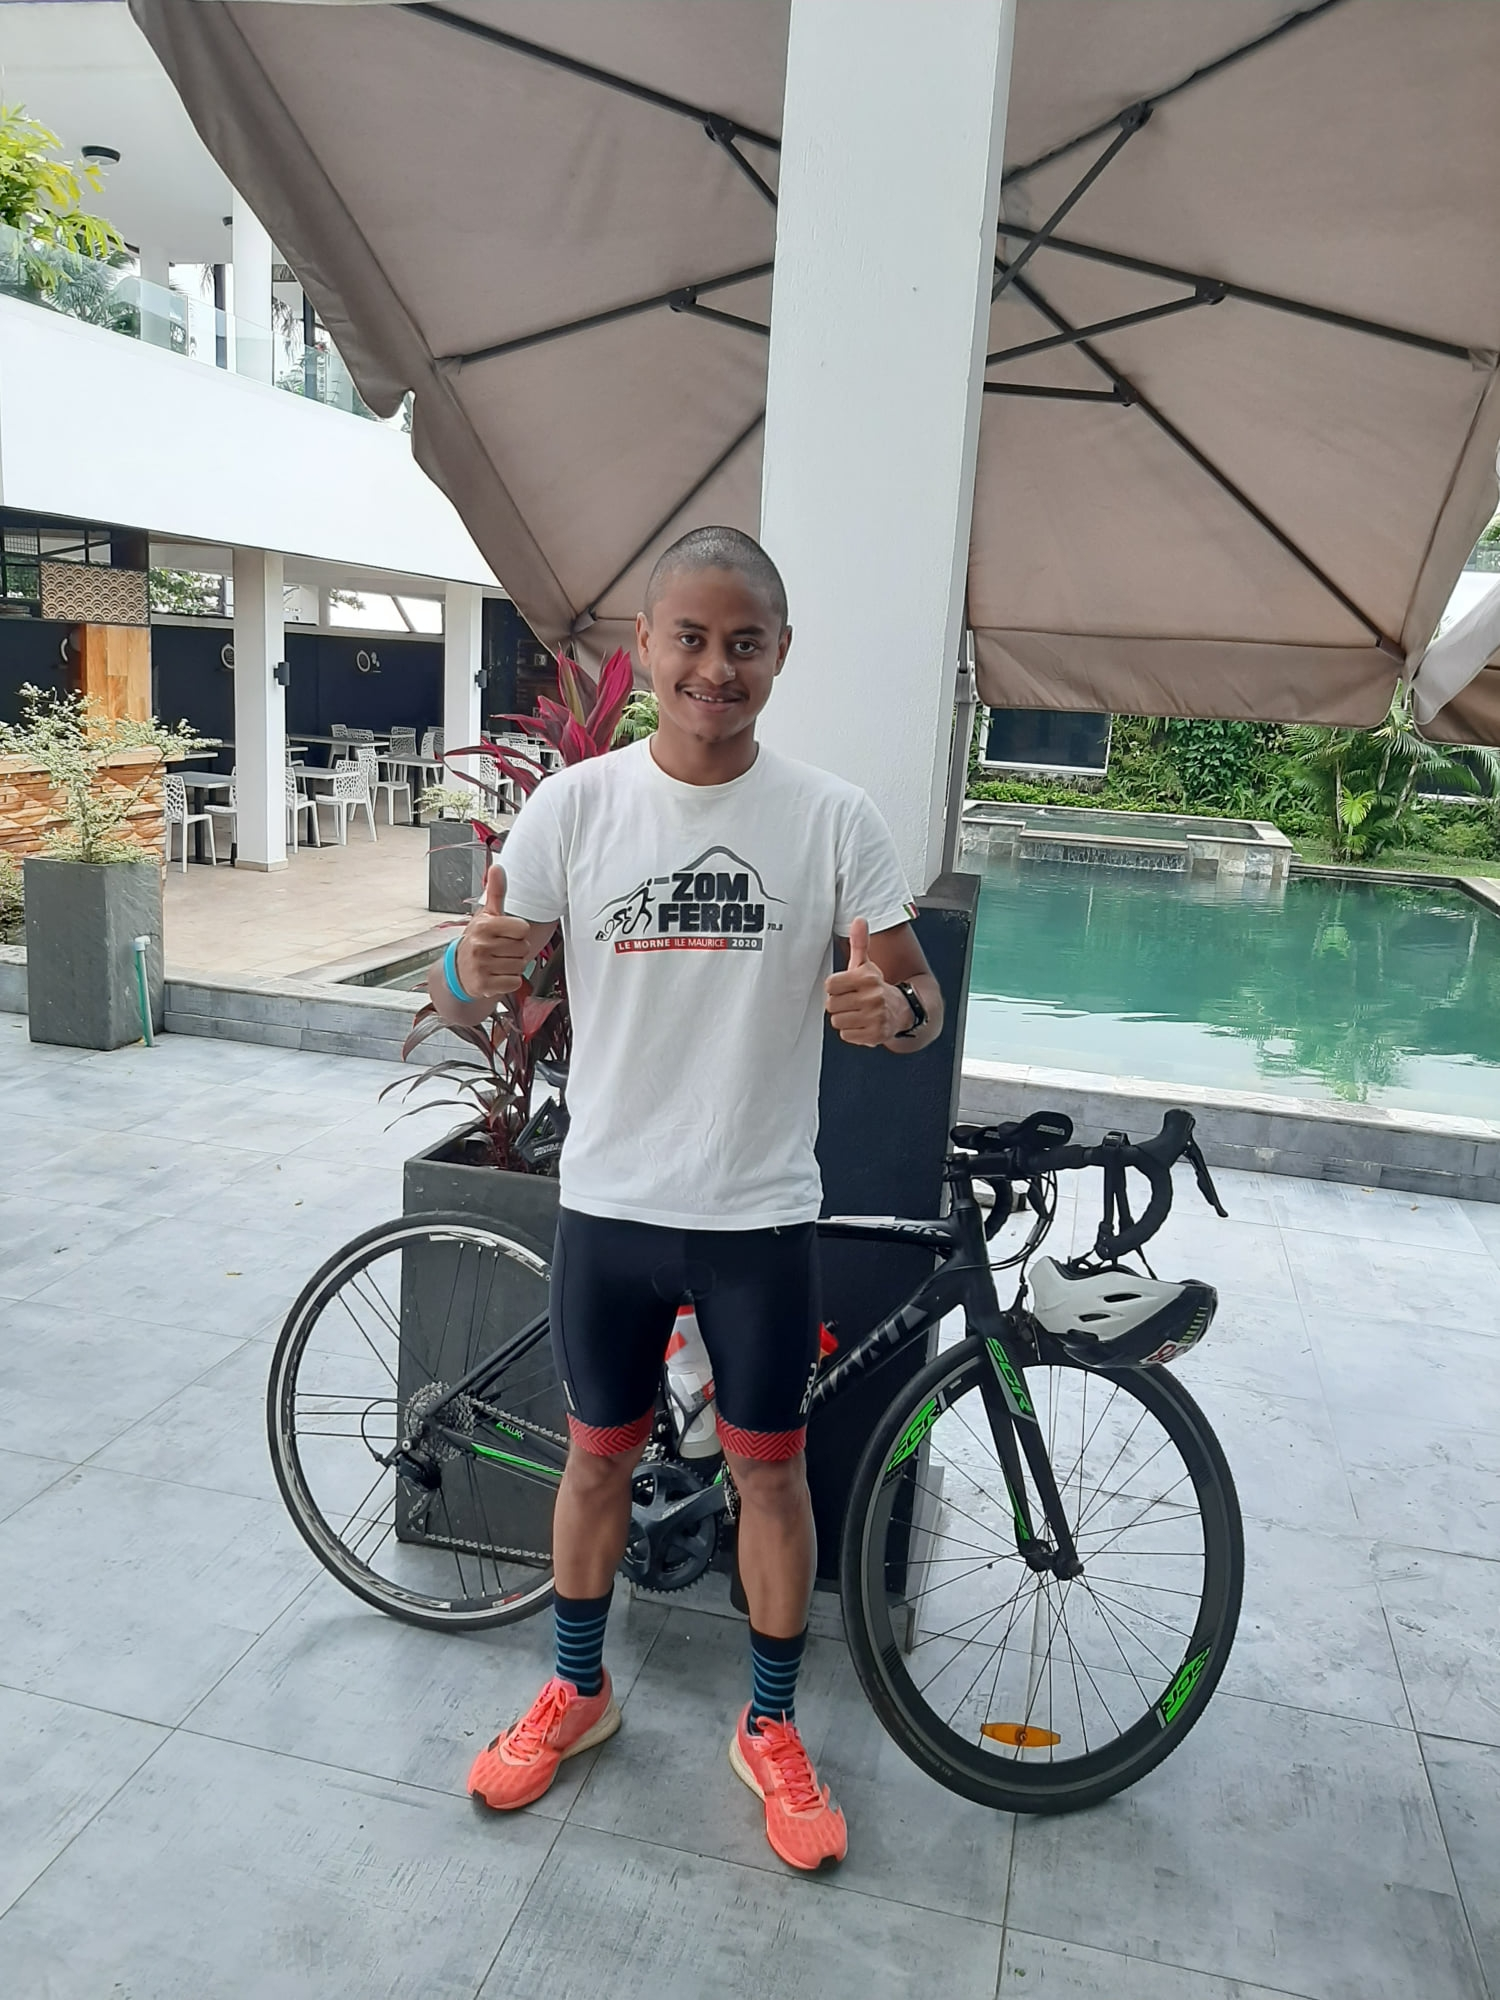
\includegraphics[width=\textwidth,height=1.04167in]{marius.jpg}

\begin{itemize}
\tightlist
\item
  Telecommunications, ESPA Alumni
\item
  Computer Science, University of Reunion Island Alumni
\item
  FaceDev Admin since 2012
\item
  Founder member of AlgoMada
\item
  Clojure dev
\item
  Computer Science Enthusiast
\item
  Current interests: Cryptocurrency, Clojure programming language
\item
  Side project: BetaX Community
\end{itemize}

\end{frame}

\begin{frame}{What is a graph?}
\protect\hypertarget{what-is-a-graph}{}

A data structure to represent link between objects. A graph is defined
by a set of nodes V and a set of edges E.

We can summarize this definition by the following formula:

\[
G = (E, V)
\]

Example:
\url{https://www.redblobgames.com/pathfinding/grids/graphs.html}

\end{frame}

\begin{frame}{What's the difference between a graph and a tree?}
\protect\hypertarget{whats-the-difference-between-a-graph-and-a-tree}{}

A graph can contain cycles (a node can be visited twice).

\end{frame}

\begin{frame}{Different type of graphs}
\protect\hypertarget{different-type-of-graphs}{}

\begin{itemize}
\tightlist
\item
  Acyclic Graph A graph that has no cycle.
\item
  Cyclic Graph A graph that has at least one cycle.
\item
  Directed Graph A graph in which edge has direction. That is the nodes
  are ordered pairs in the definition of every edge.
\item
  Undirected Graph A graph in which edge are not directed. Meaning, the
  edges are defined by an unordered pair of nodes.
\item
  Directed Acyclic Graph A graph that is both directed and acyclic.
\item
  Connected graph Every pair of nodes has a path linking them. Put in
  another way, there are no inaccessible node.
\item
  Disconnected graph A graph in which there is at least one inaccessible
  node.
\end{itemize}

\end{frame}

\begin{frame}{Different way to represent a graph}
\protect\hypertarget{different-way-to-represent-a-graph}{}

There are 2 ways to represent a graph:

\begin{itemize}
\tightlist
\item
  adjacency list For each node, provide a list of other nodes that are
  adjacent to it.
\item
  adjacency matrix A matrix construct by aligning the nodes in the row
  and the columns and putting a value if the nodes are linked by an
  edge.
\end{itemize}

\begin{figure}
\centering
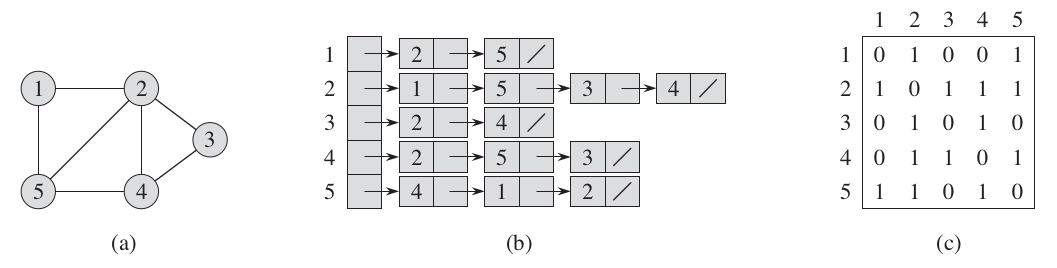
\includegraphics{graph-representation.png}
\caption{(a) Undirected graph with 5 vertices and 7 edges (b)
Adjacency-list representation (c) Adjacency-matrix representation}
\end{figure}

\end{frame}

\begin{frame}{Graph traversal algorithms}
\protect\hypertarget{graph-traversal-algorithms}{}

\begin{block}{DFS (Depth-First Search)}

A graph traversal algorithm in which one start with a root node
(arbitrarily chosen) then explore as far as possible along each branch
before backtracking.

\end{block}

\begin{block}{BFS (Breadth-First Search)}

A graph traversal algorithm in which one explore every possible node in
the current depth level before going to the next.

\end{block}

\end{frame}

\begin{frame}{BFS (Breadth-First Search)}
\protect\hypertarget{bfs-breadth-first-search-1}{}

\begin{figure}
\centering
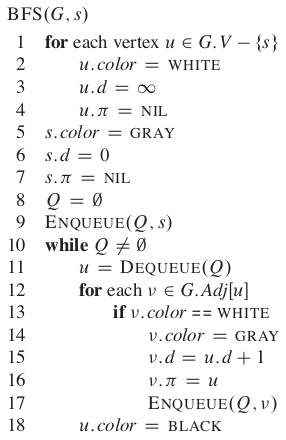
\includegraphics[width=\textwidth,height=2.60417in]{breadth-first-search-pseudocode.png}
\caption{Breadth-first search pseudo-code}
\end{figure}

\end{frame}

\begin{frame}{BFS (Breadth-First Search)}
\protect\hypertarget{bfs-breadth-first-search-2}{}

\begin{figure}
\centering
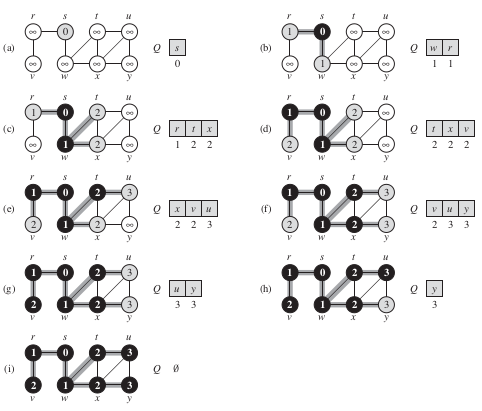
\includegraphics[width=\textwidth,height=2.60417in]{bfs-undirected-graph.png}
\caption{Operation of BFS on an undirected graph}
\end{figure}

\end{frame}

\begin{frame}{Depth-First Search}
\protect\hypertarget{depth-first-search}{}

\begin{figure}
\centering
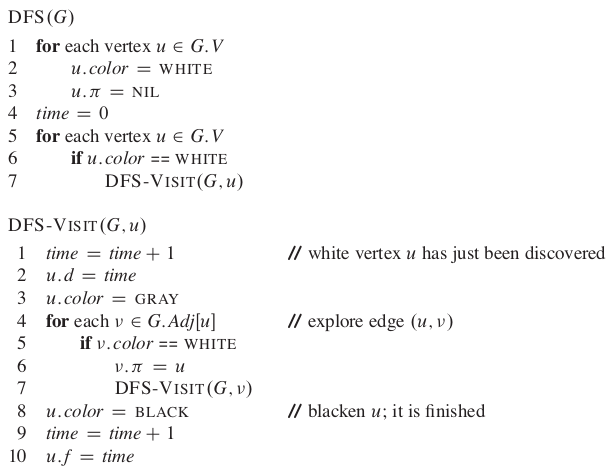
\includegraphics[width=\textwidth,height=2.60417in]{depth-first-search-pseudocode.png}
\caption{Depth-First Search Pseudocode}
\end{figure}

\end{frame}

\begin{frame}{Depth-First Search}
\protect\hypertarget{depth-first-search-1}{}

\begin{figure}
\centering
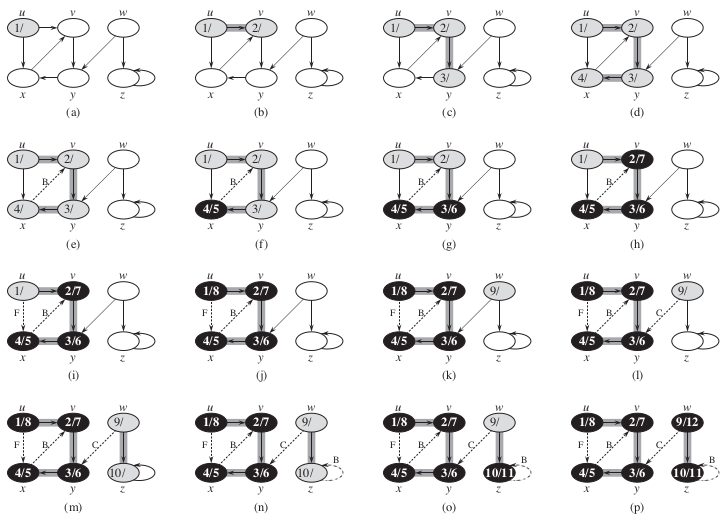
\includegraphics[width=\textwidth,height=2.86458in]{progress-dfs-directed-graph.png}
\caption{Depth-First Search progress on a directed graph}
\end{figure}

\end{frame}

\begin{frame}{Path finding algorithms}
\protect\hypertarget{path-finding-algorithms}{}

\begin{block}{A* algorithm}

A* (pronounced ``A-Star'') is a graph traversal and path-finding
algorithm. Given a source and a goal node, the algorithm find the
shortest-path (with respect to given weights) from source to goal.

\end{block}

\begin{block}{Dijkstra algorithm}

Dijkstra algorithm solves the single-source shortest-paths problem on a
weighted directed graph for the case in which all weights are
non-negative.

\end{block}

\end{frame}

\begin{frame}{Path-finding}
\protect\hypertarget{path-finding}{}

\begin{figure}
\centering
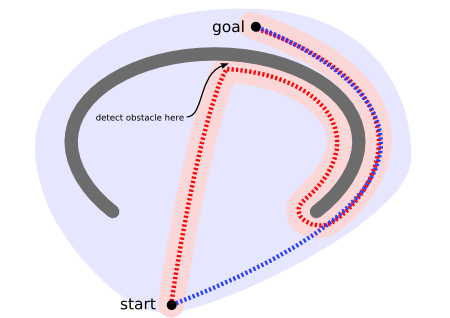
\includegraphics[width=\textwidth,height=2.60417in]{concave1.png}
\caption{Example path-finding situation}
\end{figure}

\end{frame}

\begin{frame}{Path-finding}
\protect\hypertarget{path-finding-1}{}

\begin{figure}
\centering
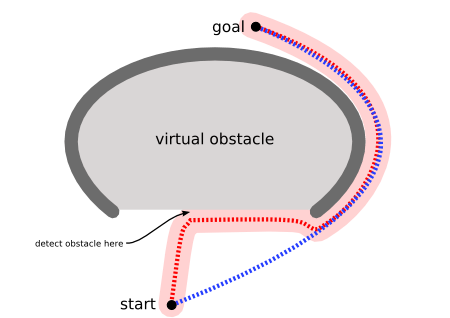
\includegraphics[width=\textwidth,height=2.60417in]{concave2.png}
\caption{Example path-finding situation}
\end{figure}

\end{frame}

\begin{frame}{A* Algorithm}
\protect\hypertarget{a-algorithm-1}{}

\begin{block}{History}

\begin{figure}
\centering
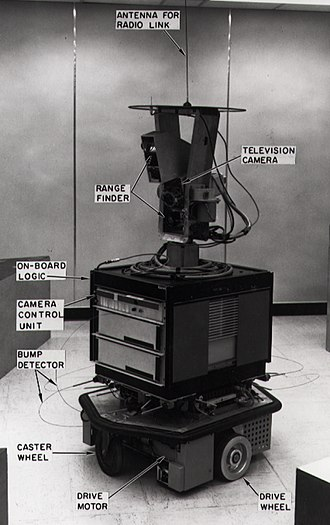
\includegraphics[width=\textwidth,height=2.60417in]{330px-SRI_Shakey_with_callouts.jpg}
\caption{A* was invented by researchers working on Shakey the Robot's
path planning.}
\end{figure}

\end{block}

\end{frame}

\begin{frame}{References}
\protect\hypertarget{references}{}

\begin{itemize}
\tightlist
\item
  https://en.wikipedia.org/wiki/A*\_search\_algorithm
\item
  http://theory.stanford.edu/\textasciitilde{}amitp/GameProgramming/AStarComparison.html
\end{itemize}

\end{frame}

\end{document}
